\subsection{Signal Start Detection}
\label{subsec:03_signalStartDetection}

As mentioned in \cref{sec:02_signalStartDetection}, the detection of the
signal start is crucial for the localization.
The implementation of the different approaches will be presented coupled with
an examination of real measurement data.
\\
To reduce undesirable effects and demonstrate the simplest form, a sinusoidal
signal of $3\si{\kilo\hertz}$ was recorded with a sample rate of $44.1\si{\kilo\hertz}$.
For the following data, the sound source was placed $2\si{m}$ in front of the robot.
\\
In order to find the time point where the signal starts, information about
smaller fractions are required.
So, the original $44100$ samples that were buffered by the
\lstinline!WhistleLocalization! module are divided into several overlapping
frames with size $256$. The computational effort raises with smaller frame size,
but delivers a higher precision in return.
In order to perform the \ac{FFT} most efficiently, the size of one frame
should be a power of 2.
To compute the energy and entropy, the frames are transformed into
frequency domain with the \ac{FFT}.
The \ac{ZCR} does not require such a transformation.
In the evaluation \cref{sec:04_signalStartDetection}, the result of the single
methods are compared to each other.
For better visualization, the following data is shortened to $2400$ samples.

\missing[]{Start detection by frequency, whistle detection}

\subsubsection*{Spectral Entropy}

The formula to calculate the spectral entropy of a signal is introduced as
\cref{eq:02_entropy} in the previous chapter.
For the entropy information, the signal must not be cleaned previously.
By looking at the derivation of the entropy, a global minimum can be found
at the starting point of the signal due to its change from noise to signal.
The starting index is therefore defined by the index of the derivation's minimum.
Of course, this approach does not work real-time but with small delay.
\Cref{fig:03_entropy} is a plot of the recorded sine signal with the corresponding
entropy.
According to the frame size, the accuracy of the start index can be increased.
However, the frame size is limited by the required number of samples for one \ac{FFT} and
its computational effort.
% -------------------------------------------------------------
\begin{figure}[ht]
	\centering
		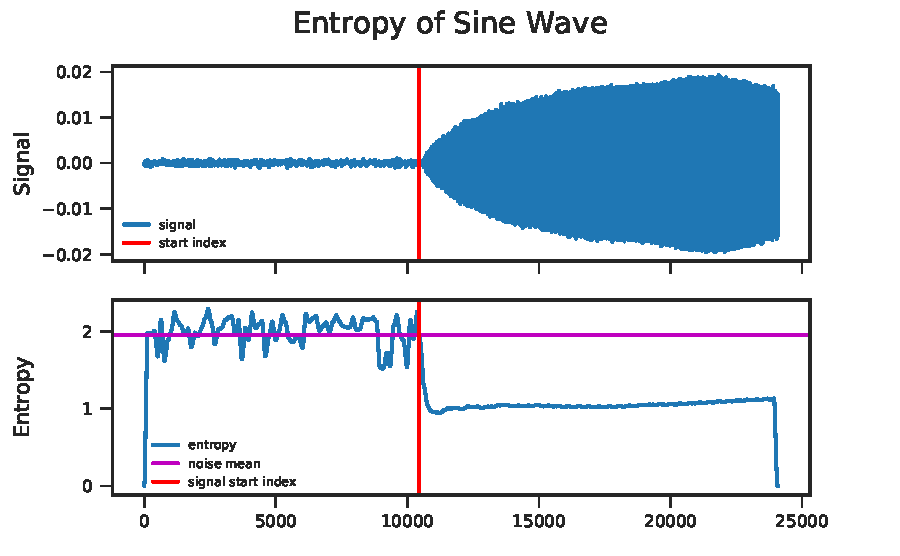
\includegraphics[]{figures/sine_entropy}
	\caption{Exemplary entropy of a sinusoidal signal with 3\si{\kilo\hertz}.}
	\label{fig:03_entropy}
\end{figure}
% -------------------------------------------------------------
In \cref{subsec:04_entropy}, the entropy outcome of a whistle sound
and its derivation is presented for evaluation.

\subsubsection*{Energy}

As mentioned above, the total signal is divided into multiple overlapping frames.
\Cref{eq:02_spectralEnergy} represents the energy of each frequency
component.
According to this, the energy of one of those frames is \cref{eq:02_energy}.
Assuming that the energy holds for the whole frame, overlapping and adding the energy
results in \cref{fig:03_energy}.
If the frequency of the examined signal is known as for the whistle, only energy values
of the relevant frequencies needs to be considered.
One downside of the energy information is that the threshold has to be adapted
manually for the related environment.
Especially at the tournament, parameters like these should be avoided and thus,
the start detection by energy is inconvenient.
% -------------------------------------------------------------
\begin{figure}[ht]
	\centering
		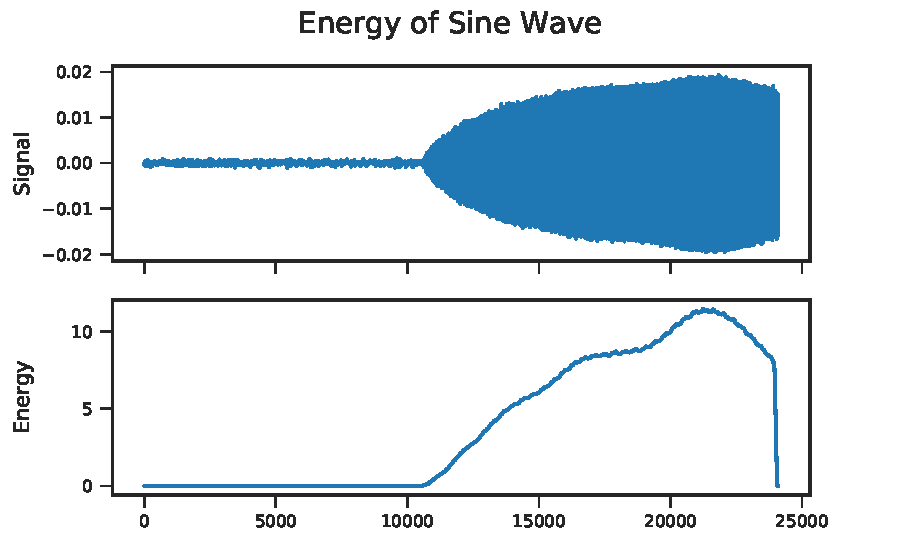
\includegraphics[]{figures/sine_energy}
	\caption{Energy of a sinusoidal signal with 3\si{\kilo\hertz}.}
	\label{fig:03_energy}
\end{figure}
% -------------------------------------------------------------

\subsubsection*{Zero Crossing Rate}

Alike the other methods, the buffered signal is divided into smaller frames
which can be set arbirary small for the \ac{ZCR} where no \ac{FFT} is necessary.
% To receive a higher accuracy, the frames of the \ac{ZCR} can be set small.
% are set to 80 samples.
In each frame, the sign changes are counted which only requires simple implementation
and computationally lightweight.
It is known that only noise is received at the beginning of the measurement and on the
contrary, signal noise is present at the end.
By comparing the mean of the received noise at the beginning of the measurement and
the mean of the signal part, a dynamic threshold can be defined and the beginning of the
signal is detectable.
In this work, the crossing of the threshold is observed from the last
value to the first.
Number of noise and signal frames are parameter values which depend
on the amount of samples and the size of the frame.
% In \cref{fig:03_zcr} and in this work, the threshold is set by multiplying the
% mean of the noise and signal mean by factor 1,25.
\begin{figure}[ht]
	\centering
		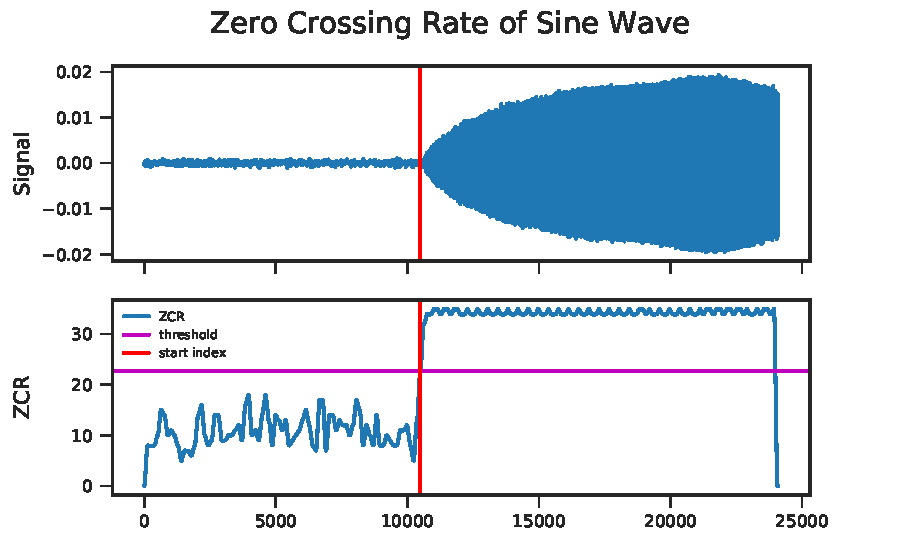
\includegraphics[]{figures/sine_zcr}
	\caption{Zero Crossing Rate of a sinusoidal signal with 3\si{\kilo\hertz}.}
	\label{fig:03_zcr}
\end{figure}
According to the circumstances, the threshold can be lowered optionally.
For real whistle data, the mean of noise and signal mean is reduced by factor 0,9 to
lower the threshold and results are shown in \cref{subsec:04_zcr}.
